Reduction Automata were introduced in \cite{dauchet:reduction}.

\Note{RA is single-ply AWEDC subject to Reduction metaconstraint (and, by
implication, Stated).}

\Note{\cite[p133]{tata} discusses the relaxation of RA to permit AWCBB-style
constraints freely; what I've called ``Deep-Reduction'' above.  This class has decidable emptyness testing.}

\subsection{Proof of Non-deterministic RA Undecidable Emptiness Testing}

\cite[Thm 4.4.7]{tata} contains a proof%
%
\footnote{Apparently first presented in \cite[Appendix
C]{jacquemard:tamodeq} and in contradiction to the statement made in
\cite[\S 4.1]{dauchet:reduction} that the proof therein, which applies to
{\em deterministic} and {\em complete} RAs, carries over to the
non-deterministic case as well.}
%
that emptiness is not decidable for the class of nondeterminstic RAs.  (This
proof generalizes to a large class of tree automata; see
\autoref{sec:tree-sepex:twocm}.)  We feel that a few words said about this
proof here may help to de-mystify it.

\begin{wrapfigure}{r}{3.5in}\centering\begin{tikzpicture}
\Tree [.h$_n$
         [.q $C_n$
            [.h$_{n-1}$ [.q $C_{n-1}$ [.h$_{n-2}$ \edge[roof];$\cdots$ ] ]
                           [.h$_{n-2}$ \edge[roof];$\cdots$ ] ] ]
         [.h$_{n-1}$
			[.q \edge[roof];$\cdots$ ]
			[.h$_{n-2}$
				[.q \edge[roof];$\cdots$ ]
				[.$\cdots$	$\cdots$ [.h$_{1}$ [.q \edge[roof];$C_1$ \# ] \# ] ]
			]
         ]
      ]
\end{tikzpicture}\end{wrapfigure}

The overall structure of the trees accepted by this construction was not
immediately obvious to at least one author of this zoo, so a schematic view
is given here.  Each h$_i$ represents the apex of {\em the same tree}
everywhere it occurs.  (\cite{tata} sometimes labels the root of the tree
``k'' and sometimes ``h$'$''; this does not appear essential to the
construction and so we simply use ``h'' pervasively.)  Every h$_i$ node
carries the trace of the first $i$ steps of execution on its right; its left
child can be thought of as the pair of the $i$-th state of the machine's
execution, denoted $C_i$, and h$_{i-1}$.  The equality constraints are
introduced only at the top and at ``q'' nodes in the tree; the state labels
are carefully constructed so that only three ranks are required to satisfy
the Reduction metaconstraint: a base rank, which includes all labels in the
$C_i$ trees is $\le$ a ``q''-state rank which includes the labels of all
``q'' and ``h'' nodes in the tree except the apex; the accepting state at
the root is the sole member of the third rank.  There will be $2^{n-i+1}$
copies of $h_i$ (or $C_i$) in a tree encoding $n$ steps.  This machine is
{\em deeply} dependent on the fact that non-determinism allows equal trees
to have several distinct runs. 
